\documentclass[20pt,margin=2in,innermargin=-12in,blockverticalspace= 2cm]{tikzposter}
\geometry{paperwidth=60in,paperheight=36in}
\usepackage[utf8]{inputenc}
\usetheme{Autumn}
\usepackage{graphicx}
\usepackage{enumitem}
\usepackage{natbib}
\bibliographystyle{econometrica}
\usepackage{amssymb}
\usepackage{pgfplots}

%%%%%%%%%%%%%%%%%%%%%%%%%%%%%%%%%%%%%%%%%
% Coe Colors
%%%%%%%%%%%%%%%%%%%%%%%%%%%%%%%%%%%%%%%%%

% Primary Colors
\definecolor{crimson}{RGB}{136, 0, 17}
\definecolor{gold}{RGB}{211, 144, 47}
% Secondary Colors
\definecolor{darkcrimson}{RGB}{133, 0, 0}
\definecolor{lightgray}{RGB}{225, 225, 225}
\definecolor{darkgray}{RGB}{128, 128, 128}

% Tertiary Colors
\definecolor{teal}{RGB}{0, 100, 125}
\definecolor{plum}{RGB}{92, 13, 52}
\definecolor{lightblue}{RGB}{105, 167, 196}
\definecolor{darkblue}{RGB}{38, 54, 92}

\definecolor{EAPviolet}{RGB}{86, 63, 70}
\definecolor{EAPgreen}{RGB}{88, 140, 126}
\definecolor{EAPyellow}{RGB}{242, 174, 114}
\definecolor{brown}{RGB}{92, 46, 0}

\definecolor{EAPred}{RGB}{136, 0, 17}
\definecolor{EAPblue}{RGB}{0, 100, 125}

\title{Green Commercial Development within Urban Environments: Theory \& Evidence}
\author{Evan Perry}
\institute{Stead Department of Business Administration \& Economics\\ Summer Research in Economics: Fellows Program}
\date{\today}


\definecolorstyle{sampleColorStyle}{
	\definecolor{colorOne}{named}{crimson}
	\definecolor{colorTwo}{named}{gold}
	\definecolor{colorThree}{named}{lightgray}
	}{
	% Background Colors
	\colorlet{backgroundcolor}{white}
	\colorlet{framecolor}{white}
	% Title Colors
	\colorlet{titlefgcolor}{black}
	\colorlet{titlebgcolor}{white}
	% Block Colors
	\colorlet{blocktitlebgcolor}{colorOne}
	\colorlet{blocktitlefgcolor}{white}
	\colorlet{blockbodybgcolor}{lightgray!50!}
	\colorlet{blockbodyfgcolor}{black}
	% Innerblock Colors
	\colorlet{innerblocktitlebgcolor}{black}
	\colorlet{innerblocktitlefgcolor}{black}
	\colorlet{innerblockbodybgcolor}{colorThree!80!white}
	\colorlet{innerblockbodyfgcolor}{black}
	% Note colors
	\colorlet{notefgcolor}{black}
	\colorlet{notebgcolor}{colorTwo!50!white}
	\colorlet{noteframecolor}{colorTwo}
}

\defineblockstyle{Slide}{
    titlewidthscale=1, bodywidthscale=1, titleleft,
    titleoffsetx=0pt, titleoffsety=0pt, bodyoffsetx=0pt, bodyoffsety=0pt,
    bodyverticalshift=0pt, roundedcorners=0, linewidth=0pt, titleinnersep=1cm,
    bodyinnersep=1cm
}{
    \ifBlockHasTitle%
        % changed "right color=..,left color=.." to "fill=blocktitlebgcolor"
        \draw[draw=none, fill=blocktitlebgcolor] 
           (blocktitle.south west) rectangle (blocktitle.north east);
    \fi%
    \draw[draw=none, fill=blockbodybgcolor] %
        (blockbody.north west) [rounded corners=30] -- (blockbody.south west) --
        (blockbody.south east) [rounded corners=0]-- (blockbody.north east) -- cycle;
}

\settitle{ \centering \vbox{
\@titlegraphic \\[\TP@titlegraphictotitledistance] \centering
\color{titlefgcolor} {\bfseries \Huge \sc \@title \par}
\vspace*{1em}
{\huge \@author \par} \vspace*{1em} {\LARGE \@institute}
%\vspace*{1em}
%\begin{tikzpicture}
%\fill[gold] (0,0) rectangle (50,.5);
%\end{tikzpicture}
}}

\tikzposterlatexaffectionproofoff
\setlength{\tabcolsep}{15pt}
\usecolorstyle{sampleColorStyle}

%\titlegraphic{
\includegraphics[width=0.07\textwidth]{CoeLogo.jpg}}
% begin document
\begin{document}

\maketitle[width = 0.7\textwidth]
\node[anchor=west] at (TP@title.west) {
\includegraphics[width=.1\textwidth]{CoeLogo.jpg}};
\node[align = center, anchor=east] at (TP@title.east) {\large Additional\\ \large Materials\\ 
\includegraphics[width=.04\textwidth]{qr.png}};
%\node[anchor=south] at (TP@title.east) {Additional Materials};

\centering

\begin{columns}

\column{0.2}

\block{Research Goal}{
\vspace*{-1.3cm}
\hspace*{-1.18cm}

\begin{tikzpicture}
	\fill[gold] (0,0) rectangle (25.8,.3);
\end{tikzpicture}
~

\vspace{-.5cm}
The research objective is to explore and explain the spatial distribution of green commercial buildings within cities by first developing a spatial equilibrium model for commercial green development and then testing the model's prediction.
}

\block{Motivation \& Related Literature}{
\vspace*{-1.3cm}
\hspace*{-1.18cm}

\begin{tikzpicture}
	\fill[gold] (0,0) rectangle (25.8,.3);
\end{tikzpicture}

\vspace{-.5cm}
\subsection*{Why Green Buildings?}

\begin{itemize}
	\item Buildings account for 30\% of all greenhouse gas emissions in the US \citep{rfftoolkit}
	\item Investment in energy-efficient buildings can be a win-win: firms reduce energy expenses and policy makers achieve lower greenhouse gas emissions
	\item Major policy proposals like the American Jobs Plan contain funding for investment in green infrastructure, particularly homes and commercial buildings
	\item There is a need for formal theory with empirical support to consider policy obstacles and strategy
\end{itemize}

\subsection*{The Adoption Decision}
\begin{itemize}
	\item \cite{allcott2012there} utilize a simple model for the adoption of energy-efficient technologies and introduce issues of energy expense salience in adoption
	\item \cite{bansal2000companies} provide a qualitative analysis of firm attributes associated with greater ecological responsiveness, and thus greater adoption of green technologies
\end{itemize}

\subsection*{The Location Decision}

\begin{itemize}
	\item \cite{glaeser2008cities} refines and applies earlier spatial equilibrium models to describe how workers, firms, and developers interact to determine local wages, rents, and housing supply
	\item \cite{gaubert2018firm} builds heterogeneous firms and evaluates how these firms will choose to locate across different cities based on their sectoral agglomeration economies
\end{itemize}
}

\block{The Model: Environment}{
\vspace*{-1.3cm}
\hspace*{-1.18cm}

\begin{tikzpicture}
	\fill[gold] (0,0) rectangle (25.8,.3);
\end{tikzpicture}

\begin{itemize}
	\item Consider one city with many neighborhoods
	\item Before firms locate, neighborhoods differ only in their number of workers $N$
	%\item Open world: firms can move and trade freely
	\item Firms can move/trade freely (an open world) and all decisions occur in the same period (static model)
	\item Two Actors: Firms  and developers
	\item Want to determine (1) the adoption decision, (2) the location decision
\end{itemize}

}

\column{0.2}

\block{The Model: Actors \& Behavior}{
\vspace*{-1.24cm}
\hspace*{-1.18cm}

\begin{tikzpicture}
	\fill[gold] (0,0) rectangle (25.8,.3);
\end{tikzpicture}

\vspace{-1em}
\subsection*{Firms}

%\begin{itemize}
%	\item Heterogeneous in:
%	\begin{enumerate}
%		\item Agglomeration economies
%		\item Ecological Responsiveness
%	\end{enumerate}
%	\item Profit maximizing:
%\end{itemize}
Firms differ along two dimensions: (1) ecological responsiveness, and (2) agglomeration economies. %The firm's goal is to choose the combination of labor, real estate, the design of that real estate, and neighborhood to maximize its profits. Formally,  
The firm is profit maximizing:
$$\max_{L, R, d, N} \left\{ A \psi(\alpha_i, N) \lambda(\theta_j, d) L^\beta R^\gamma \overline{K}^{1-\beta-\gamma} - WL - p_d R - k_{ij}\right\}.$$
\begin{center}
\begin{tabular}{c p{17cm}}
$A$ & Raw productivity\\
$\alpha_i$ & Agglomeration ranking for industry $i$; \newline{high $\alpha_i \Rightarrow$ high agglomeration} \\
$\psi(\alpha_i, N)$  & Agglomeration effect for firm type $i$ in neighborhood $N$ \citep{gaubert2018firm}\\
$\theta_j$ & Ecological response ranking for type $j$;\newline{high $\theta_j \Rightarrow$ high ecological response}\\ 
$\lambda(\theta_j, d)$   & Ecological response for firm type $j$ with building design $d$\\
$L$  & Labor (in workers)\\
$R$  & Commercial real estate (in square feet)\\
$\overline{K}$  & Fixed capital inputs\\
$W$  & Wage\\
$p_d$  & Price per square foot of commercial real estate with design $d$\\
$k_{ij}$  & Entrance costs to firm type $ij$
\end{tabular}
\end{center}

\subsection*{Developers}

%Developers competitively bid on all commercially developable land in a neighborhood, resulting in a single developer in each neighborhood. %The developer's goal is to choose the height and land footprint for all green and brown (non-green) construction in the neighborhood that will maximize the sum of its profits from green and brown construction. That is,

There is a single, profit-maximizing developer in each neighborhood.
$$\max_{h_g, h_b,\ell_g, \ell_b} \left\{ \pi_g(h_g, \ell_g) + \pi_b(h_b, \ell_b)\right\} \hspace{2cm}\mathrm{s.t.}\hspace{2cm} \bar{\ell} = \ell_g + \ell_b$$
where for building design $d\in \{g\textcolor{black!60!}{reen}, b\textcolor{black!60!}{rown}\}$,
$$\pi_d(h_d, \ell_d) = p_d h_d \ell_d - c_d h_d^\eta \ell_d - p_\ell \ell_d.$$
\begin{center}
\begin{tabular}{c p{17cm}}
	$h_d$ & Height of buildings with design $d$\\
	$\ell_d$ & Land allocation for buildings with design $d$\\
	$\bar{\ell}$ & Total land available for commercial development\\
	$p_d$ & Price of commercial real estate with design $d$ per square foot\\
	$c_d$ & Material cost per square foot (for single story) with design $d$; $c_g > c_b$\\
	$p_\ell$ & Price of land per square foot\\
	$\eta$ & Upward friction parameter of building, $\eta > 1$\\
\end{tabular}
\end{center}

}


\block{Agglomeration \& Ecological Response}{
\vspace*{-1.3cm}
\hspace*{-1.18cm}

\begin{tikzpicture}
	\fill[gold] (0,0) rectangle (25.8,.3);
\end{tikzpicture}

\vspace{1em}
%\bigskip
\textit{What drives agglomeration and ecological responsiveness?}
\begin{itemize}
	\item Importance of connections with similar firms  \citep{bansal2000companies}%: Firms reliant on similar firms receive a higher benefit from agglomeration. This connection leads to rapid diffusion of green improvements \citep{bansal2000companies}.
	\item Importance of human connections \citep{kok2012diffusion} %: These firms can profit more from knowledge spillovers, making yielding higher agglomeration effects. Reputation effects are especially strong, so firms benefit more from a green reputation \citep{kok2012diffusion}.
\end{itemize}

%We do not model these determinants directly, but instead make the assumption that firms with high agglomeration effects (high $\alpha_i$) are more likely to have a ecological responsiveness ($\theta_j$) that will trigger investment in green real estate. 

Assume in higher agglomeration industries firms have higher ecological responsiveness types that induce them to adopt green buildings more frequently. Formally, for firms 1 and 2 with $\alpha_1 < \alpha_2$, then 
$$\Pr\{\theta_1 > \theta^*\mid \alpha_1\} < \Pr\{\theta_2 > \theta^*\mid \alpha_2\}.$$

}

\column{0.2}

\block{Equilibrium}{
\vspace*{-1.32cm}
\hspace*{-1.18cm}

\begin{tikzpicture}
	\fill[gold] (0,0) rectangle (25.8,.3);
\end{tikzpicture}

\vspace{-1em}
\subsection*{Green Building Adoption}

Firms will purchase and the developer will build green real estate if and only if the adoption condition holds:
$$\frac{\lambda(\theta_j, g)}{\lambda(\theta_j, b)} > \left(\frac{c_g}{c_b}\right)^\frac{\gamma}{\eta}.$$
With the assumptions we have made about $\lambda$, this implies there exists a threshold green benefit type $\theta^*$.
% such that for any green benefit types 1 and 2, $\theta_1 < \theta^* < \theta_2$ implies that firm type 1 will never purchase green real estate and firm type 2 will always purchase green real estate.

\subsection*{Firm Sorting}

%Spatial equilibrium guarantees that firms with identical agglomeration types are indifferent between all neighborhoods they can afford to locate in. Then
Type $ij$ firms will locate in every neighborhood in the set of optimal neighborhoods defined by,
$$N^*(\alpha_i, \theta_j) = \left\{ N\in \mathcal{N} \mid p_d^*(N, \alpha_i, \theta_j) \geq p_d^*(N, \alpha_k, \theta_j), \forall k \in \mathcal{I}\right\},$$
where $\mathcal{N}$ is the support of neighborhoods and $\mathcal{I}$ is the set of all agglomeration types. This brings us to the central claim.
%Firms with high agglomeration effects will occupy denser (higher $N$) neighborhoods as they are able to leverage this density better than low agglomeration effect firms.

\vspace{1em}
\textbf{Claim}: \textit{High agglomeration effect firms will locate in worker-dense neighborhoods and occupy green buildings more frequently.}

}

%\colorlet{blockbodybgcolor}{white}
\block{}{
%\vspace*{-1.3cm}
%\hspace*{-1.18cm}
%\begin{tikzpicture}
%	\fill[gold] (0,0) rectangle (25.8,.3);
%\end{tikzpicture}
%
%\vspace{.5em}
\centering
\textsc{Figure 1: Example with Two Agglomeration Types}
\vspace{2em}

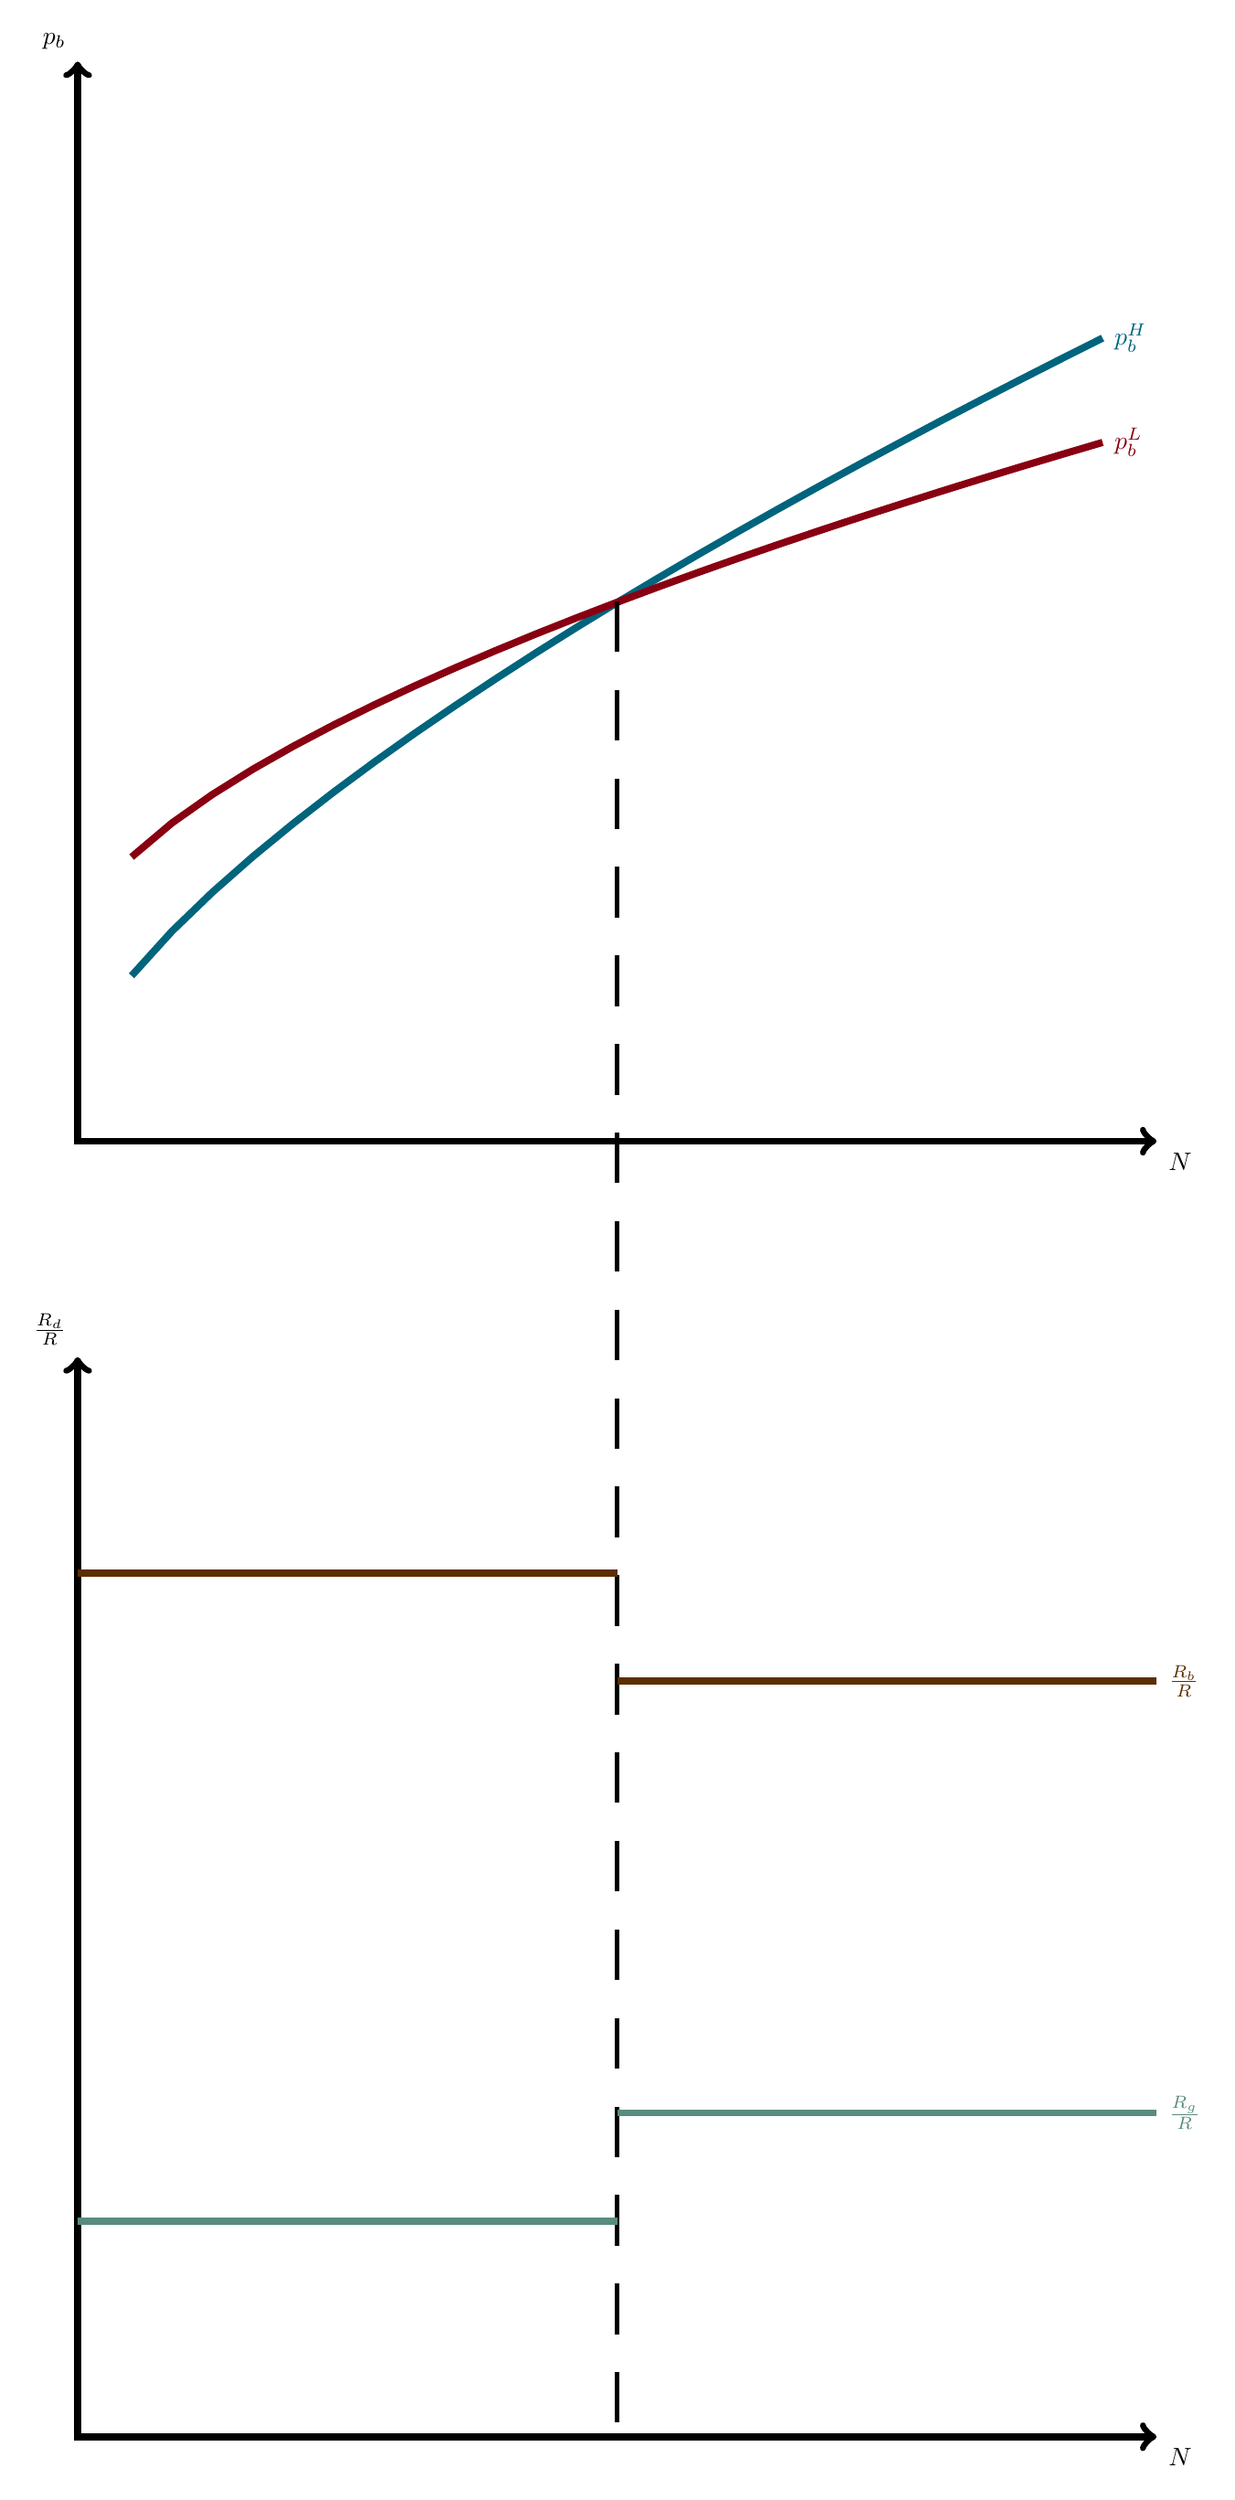
\begin{tikzpicture}[scale = 1.5]
	\draw[line width=1mm, <->] (10, 0) node[below right]{$N$} -- (0,0) -- (0,10) node[above left]{$p_b$};
	\draw[line width=1mm, <->] (10, -12) node[below right ]{$N$} -- (0,-12) -- (0,-2) node[above left]{$\frac{R_d}{R}$};
	\draw[line width=1mm, EAPblue][domain = 0.5:9.5] plot (\x, {1.4* \x^(0.7)+.67}) node[right]{$p_b^H$};
	\draw[line width=1mm, EAPred][domain = 0.5:9.5] plot (\x, {1.2*\x^(0.6) + 1.84}) node[right]{$p_b^L$};
	\draw[line width=0.7mm, dash pattern=on 20pt off 15pt,] (5,5) -- (5,-12);
	\draw[line width=1mm, brown] (0,-4) -- (5,-4);
	\draw[line width=1mm, brown] (5,-5) -- (10,-5) node[right]{$\frac{R_b}{R}$};
	\draw[line width=1mm, EAPgreen] (0, -10) -- (5, -10);
	\draw[line width=1mm, EAPgreen] (5,-9) -- (10, -9) node[right]{$\frac{R_g}{R}$};
\end{tikzpicture}

}
%\colorlet{blockbodybgcolor}{lightgray!30!}

\column{0.2}

\block{Data}{
\vspace*{-1.3cm}
\hspace*{-1.18cm}

\begin{tikzpicture}
	\fill[gold] (0,0) rectangle (25.8,.3);
\end{tikzpicture}

%Estimating the model directly would require firm-level data on green responsiveness and agglomeration effects on firms. This data does not exist, so we turn to data on the green building stock, cellphone data, and census tract data. All data is aggregated at the census tract level.
%
%\qquad Data on green buildings comes from the Energy Star Program and the Leadership in Energy and Environmental Design (LEED) program. Address data is geolocated and aggregated at the the census tract level. We use smartphone data from SafeGraph to find the number of cellphones in the SafeGraph database that stopped in the census tract during working hours in February 2019. This is taken as a proxy for the number of workers in each census tract. Demographic data comes from the census.

\begin{itemize}
	\item Data do not allow us to test the model precisely
	\item Instead, verify the claim that firms in worker-dense neighborhoods go green more often 
	\item Green building data: Clean and merge data sets $\rightarrow$ geolocate addresses $\rightarrow$ match to Census tracts $\rightarrow$ calculate count of green buildings and total green space for each Census tract
	\begin{enumerate}
		\item Energy Star Program
		\item Leadership in Energy and Environmental Design (LEED)
	\end{enumerate}
	\item Worker data: Use cellphone data from SafeGraph to proxy the number of workers in each neighborhood (from February 2019)
	\item Use 2019 Census tracts as the unit of analysis
\end{itemize}

}

\block{Empirics}{
\vspace*{-1.3cm}
\hspace*{-1.18cm}

\begin{tikzpicture}
	\fill[gold] (0,0) rectangle (25.8,.3);
\end{tikzpicture}

\begin{itemize}
	\item For ease, restrict the sample to just those Census tracts with at least one green commercial building
	\item Estimate the following model for the log of green real estate $R_g$ (in sq. ft.) in neighborhood $i$ in city $n$,
	$$\log(R_g)_{in} = \alpha + \beta N_i + \gamma \textbf{X}_i+ \sum_{n = 1}^{N} \left[ \delta_n \log\left(\frac{N_i}{\ell_i}\right) c_n\right] + \varepsilon_{in}$$
	\item $N_i$ is the number of workers proxy, $\textbf{X}_i$ is a vector of neighborhood characteristics, and $c_n$ is a dummy variable for city $n$
	\item $\delta_n$ is the percent change in green real estate for a 1\% increase in worker density
	%\item R$^2$ is somewhat low, but without firm level data this should be expected
	\item Distribution of the $\widehat{\delta}_n$'s in Figure 2 provides evidence that within cities, worker-dense neighborhoods have more green commercial real estate%, consistent with a relationship between agglomeration, ecological responsiveness, and the predicted sorting behavior
\end{itemize}

\vspace{1.25em}
\centering
\textsc{Table 1: Agglomeration \& Green Space}
\begin{tabular}{@{\extracolsep{5pt}}lccc} 
\\[-1.8ex]\hline 
\hline \\[-1.8ex] 
\\[-1.8ex] & \multicolumn{3}{c}{Log Green Real Estate (sq. ft.)} \\ 
\\[-1.8ex] && (1) & (2)\\ 
\hline \\[-1.8ex] 
Log Number of Workers && 3.213$^{**}$ & 3.158$^{**}$ \\ 
  && (0.038) & (0.039) \\ 
  && & \\ 
 Log Median Housing Value &&  & 1.228$^{**}$ \\ 
  &&  & (0.051) \\ 
  && & \\ 
 Log Median Resident Age &&  & $-$0.889$^{**}$ \\ 
  &&  & (0.155) \\ 
  && & \\ 
 Log Worker Density - City && \checkmark  &  \checkmark \\ 
  && & \\ 
Observations && 34,285 & 33,332 \\ 
R$^{2}$ && 0.263 & 0.277 \\ 
Adjusted R$^{2}$ && 0.258 & 0.272 \\ 
\hline \\[-1.8ex] 
\textit{Notes:} & \multicolumn{3}{l}{$^{*}$Sig. at 5\% level; $^{**}$Sig. at 1\% level} \\
\end{tabular} 

}

\column{0.2}

%\colorlet{blockbodybgcolor}{white}

%\block{}{
\block{Estimates}{
\vspace*{-1.3cm}
\hspace*{-1.18cm}

\begin{tikzpicture}
	\fill[gold] (0,0) rectangle (25.8,.3);
\end{tikzpicture}

\centering
\vspace{1em}
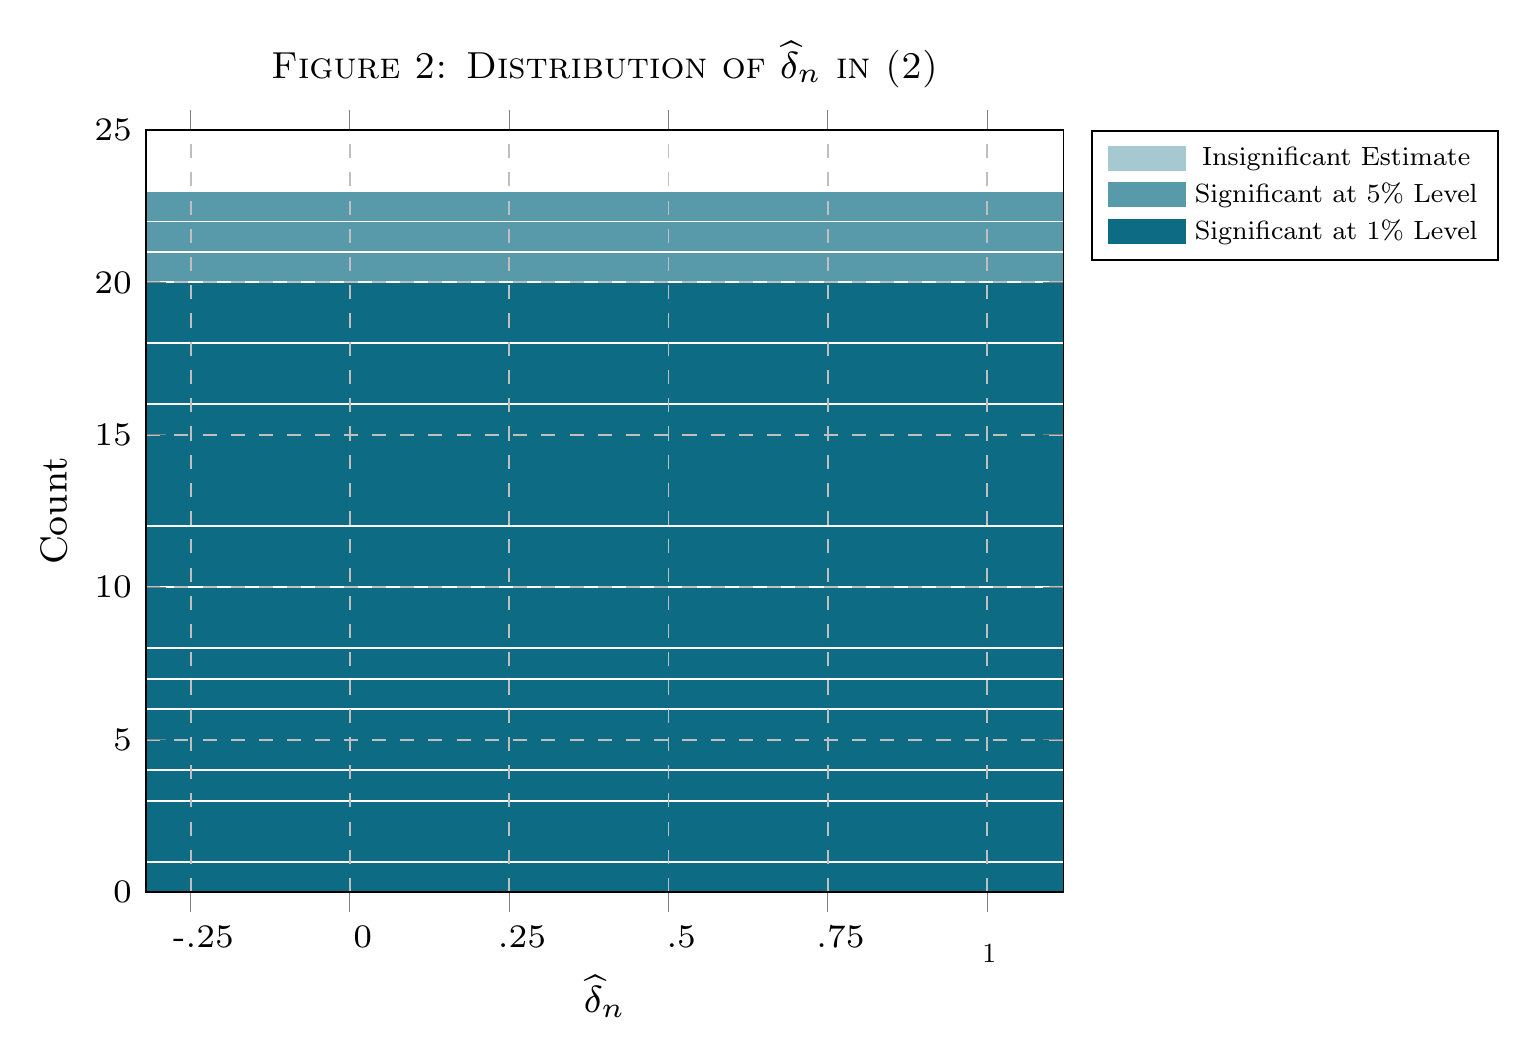
\begin{tikzpicture}[scale = 1.7]
\footnotesize
\begin{axis}[
	title={\textsc{Figure 2: Distribution of $\widehat{\delta}_n$ in (2)}},
	ybar interval, 
	bar shift=2.5pt,
	ymax=25, 
	ymin=0, 
    xlabel={$\widehat{\delta}_n$},
    ylabel={Count},
	xtick={-.25, 0, .25, .5, .75, 1},
	xticklabels = {-.25, 0, .25, .5, .75, 1},
	xticklabel style = {xshift=-0.5cm},
%    legend style={at={(0.5,-0.1)},
	legend pos = outer north east,
    ymajorgrids=true,
    grid style=dashed,
    % only marks,
    %every axis plot/.append style={ultra thick},
    ticklabel style = {font=\scriptsize},
    area style,
    legend style={nodes={scale=0.7, transform shape}}
]
\addplot+[ybar, bar width = 6, mark=no, color=white, fill=EAPblue!35!] coordinates {(-0.2,1)(-0.15,4)(-0.1,4)(-0.05,8)(0,6)(0.05,14)(0.1,13)(0.15,20)(0.2,17)(0.25,23)(0.3,23)(0.35,19)(0.4,21)(0.45,12)(0.5,12)(0.55,10)(0.6,8)(0.65,3)(0.7,4)(0.75,1)(0.8,1)(0.85,0)(0.9,1)(0.95,1)(1,0)};
\addplot+[ybar,bar width = 6,  mark=no, color=white, fill=EAPblue!65!] coordinates { (0.1,4)(0.15,11)(0.2,11)(0.25,22)(0.3,23)(0.35,19)(0.4,21)(0.45,12)(0.5,12)(0.55,10)(0.6,8)(0.65,3)(0.7,4)(0.75,1)(0.8,1)(0.85,0)(0.9,1)(0.95,1)(1,0)};
\addplot+[ybar,bar width = 6,  mark=no, color=white, fill=EAPblue!95!] coordinates {(0.1,3)(0.15,7)(0.2,6)(0.25,16)(0.3,20)(0.35,18)(0.4,20)(0.45,12)(0.5,12)(0.55,10)(0.6,8)(0.65,3)(0.7,4)(0.75,1)(0.8,1)(0.85,0)(0.9,1)(0.95,1)(1,0)};
\legend{Insignificant Estimate, Significant at 5\% Level, Significant at 1\% Level};
\end{axis}
\node at (6.3,-.46) {\normalsize 1};
\end{tikzpicture}
}

%\colorlet{blockbodybgcolor}{lightgray!30!}

\block{Takeaways \& Policy Implications}{
\vspace*{-1.3cm}
\hspace*{-1.18cm}

\begin{tikzpicture}
	\fill[gold] (0,0) rectangle (25.8,.3);
\end{tikzpicture}

\begin{itemize}
	\item Agglomeration effects and ecological responsiveness are driven by similar economic forces
	\item The model suggests green commercial development will be concentrated in worker-dense neighborhoods, and we demonstrate empirical support for this claim
	\item In the model, adoption is based on firm type, not location -- this implies effective policy targets firms with low ecological responsiveness, not places with few green buildings
\end{itemize}

}

\block{Acknowledgments}{
\vspace*{-1.3cm}
\hspace*{-1.18cm}

\begin{tikzpicture}
	\fill[gold] (0,0) rectangle (25.8,.3);
\end{tikzpicture}

\vspace{1em}
This research benefited from the invaluable comments of the students in the Spellman Fellows Program and members of the Coe College Economics faculty: Ryan Baranowski, Rick Eichhorn, and Chelsea Lensing. I am especially indebted to my faculty research advisor, Drew Westberg. Generous financial support from the Spellman Fund made this research possible.
}

\block{References}{
\vspace*{-1.3cm}
\hspace*{-1.18cm}

\begin{tikzpicture}
	\fill[gold] (0,0) rectangle (25.8,.3);
\end{tikzpicture}

\renewcommand\refname{}
\vspace{-2.4cm}
\small
\bibliography{References}
}


\end{columns}

%\node[text width=10cm,above right] at (60, -40){$^*$ eaperry19@coe.edu};

\end{document}